\documentclass[11pt,a4paper]{article}
\usepackage[T1]{fontenc}
\usepackage[utf8]{inputenc}
\usepackage[ngerman]{babel}
\usepackage[margin=2.5cm]{geometry}
\usepackage[hidelinks]{hyperref}
\usepackage{graphicx}
\setlength{\parindent}{0pt}
\begin{document}
\begin{center}
  {\Large\textbf{Webtechnologien -- Übungsblatt 2}}
\end{center}
\section*{Aufgabe 1: JavaScript Basics, Scopes, Equality}
\textbf{Aufgabe:} Das Moodle-Quiz zu JavaScript-Konzepten absolvieren
und einen Screenshot der erreichten Punkte abgeben.

\medskip
\textbf{Ergebnis:} Quiz in Moodle (H5P) abgeschlossen,
\textbf{40 von 49 Punkten}.

\begin{center}
  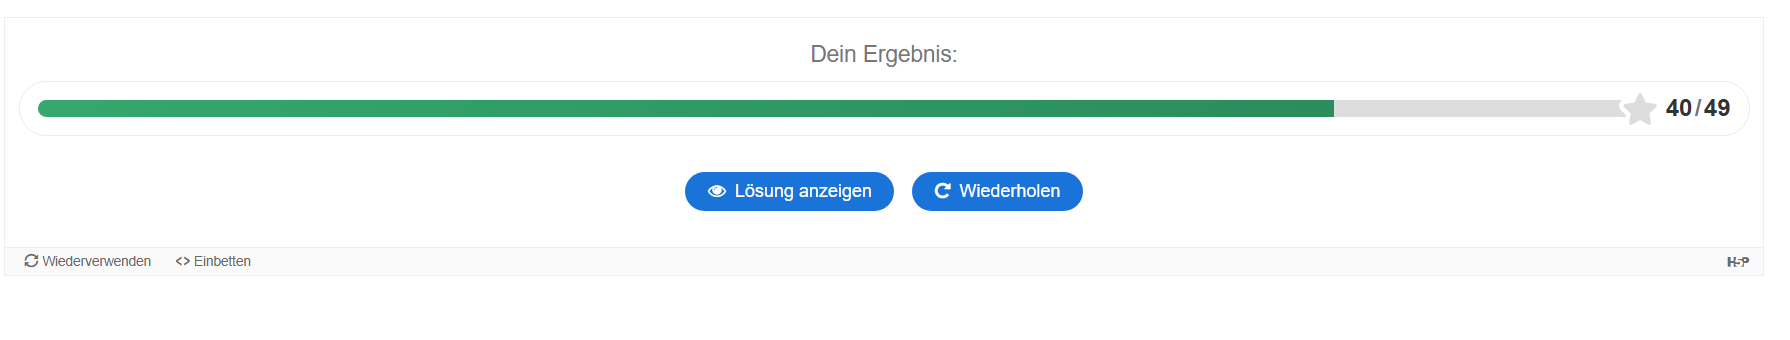
\includegraphics[width=\textwidth]{quiz-ergebnis.png}
\end{center}

\textbf{Datei:} Der Screenshot liegt zusätzlich als
\texttt{quiz-ergebnis.png} bei.

\medskip
{\small \textbf{Hilfsmittel:} Quiz selbst gelöst; Claude Code (Claude Opus 5.5) nur für die Dokumentation.}
\end{document}
